\documentclass[ngerman,aspectratio=169]{beamer}
\usepackage[utf8]{inputenc}

\usepackage[binary-units=true]{siunitx}
\usepackage[german=quotes]{csquotes}
\usepackage[nooldvoltagedirection]{circuitikz}
\usepackage[outline]{contour}
\usepackage[shorthands=off,ngerman]{babel}
\usepackage[style=iso-numeric,minnames=1,maxnames=3,giveninits,uniquename=init]{biblatex}
\usepackage[T1]{fontenc}
\usepackage{adjustbox}
\usepackage{amsmath}
\usepackage{booktabs}
\usepackage{caption}
\usepackage{datetime}
\usepackage{environ}
\usepackage{fontawesome5}
\usepackage{graphicx}
\usepackage{hyperref}
\usepackage{pgfplots}
\usepackage{spreadtab}
\usepackage{tabularx}
\usepackage{textcomp}
\usepackage{tikz}
\usepackage{xcolor}
\usepackage{appendixnumberbeamer}

\addbibresource{references.bib}
\captionsetup{justification=centering,font=footnotesize}
\contourlength{0.7pt}
\graphicspath{{images/} {matlab/}}
\pgfplotsset{width=9cm,compat=newest}
\setlength{\bibhang}{0cm} % left-align bibliography
\sisetup{locale = DE}
\tikzset{>=Stealth}
\usetheme[progressbar=frametitle]{metropolis}
\usetikzlibrary{angles,arrows.meta,calc,math,positioning,shadows,shapes.misc,tikzmark,trees,quotes}
\tikzset{
  invisible/.style={opacity=0},
  visible on/.style={alt={#1{}{invisible}}},
  alt/.code args={<#1>#2#3}{%
    \alt<#1>{\pgfkeysalso{#2}}{\pgfkeysalso{#3}} % \pgfkeysalso doesn't change the path
  },
}

\DefineBibliographyStrings{ngerman}{
    andothers = {{et\,al\adddot}},
    online = {Online},
}

\title{Passivradar}
\subtitle{Grundlagen der Signalverarbeitung}
\date{Jannuar 2021}
\author{Andreas Baulig}
\institute{Hochschule Esslingen}
\logo{
\includegraphics[height=1cm]{hs-esslingen_logo.png}}

\newcommand{\nologo}{\setbeamertemplate{logo}{}}

\begin{document}

\frame{\titlepage}

{
  \section*{Inhalt}
  \nologo{}
  \begin{frame}[allowframebreaks]
    \frametitle{Inhalt}
    \tableofcontents
  \end{frame}

  % !TeX root = ../beamer.tex
\section{Was ist Passiv Radar}

\begin{frame}
    \frametitle{Was ist Radar}

    \begin{columns}
        \begin{column}{0.6\textwidth}
            \begin{itemize}
                \item \textbf{RA}dio \textbf{D}etection and \textbf{R}anging
                \item Messung von \textbf{Entfernung} und \textbf{Geschwindigkeit}
                      \begin{itemize}
                          \item<3-> Zeitversatz \(\tau\)
                          \item<3-> Frequenzversatz \(f_{d}\)
                      \end{itemize}
            \end{itemize}
        \end{column}
        \begin{column}{0.4\textwidth}
            \begin{figure}
                \centering
                \begin{tikzpicture}
                    
\def\tickamp{0.025cm}
\def\tickseg{0.5cm}
\node [label={below:Radar}] (radar) at (0,0) {\Huge\faSatelliteDish};

\node [label={above:Target}] (target) at (3,3) {\Huge\faPlane};

\draw [visible on=<1>,decorate,decoration={expanding waves,angle=6,segment length=3pt},blue!60] (radar) -- node [fg] {\small\contourlength{2pt}\contour{bg}{Pulse}} (target);

\draw [visible on=<2->,decorate,decoration={expanding waves,angle=60,segment length=6pt},red!60] (target) -- node [fg] {\small\contourlength{2pt}\contour{bg}{Echo}} (radar);

                \end{tikzpicture}
            \end{figure}
        \end{column}
    \end{columns}
\end{frame}

\begin{frame}
    \frametitle{Was heißt Passiv?}

    \begin{columns}
        \begin{column}{0.6\textwidth}
            \begin{itemize}
                \item Beleuchtung durch Sender in der \textbf{Umgebung}
                \item Operator hat \textbf{keine Kontrolle} über Beleuchter
                \item Beleuchter und Empfänger sind \textbf{räumlich getrennt}
            \end{itemize}
        \end{column}
        \begin{column}{0.4\textwidth}
            \begin{figure}
                \centering
                \resizebox{\linewidth}{!}{
                    \begin{tikzpicture}
                        \newcommand\drawTopology[4]{
    \coordinate (rx1_coord) at (-2,0);
    \coordinate (tx1_coord) at (2,0);
    \coordinate (target_coord) at (1.25,3);

    \node at (tx1_coord) [text width=0.5cm,text height=1cm] (tx) {};
    \node at (tx1_coord) [antenna,scale=0.5,below=-0.5cm] {};
    \path let \p1=(tx.north west), \p2=(tx.south east), \p3=(tx) in [label={below:Receiver}] ({\x3-0.4cm},\y1) rectangle ({\x3+0.4cm},\y2) node [below] at (\x3,\y2) {Illuminator};

    \node at (rx1_coord) [text width=0.5cm,text height=0.75cm] (rx) {};
    \node at (rx1_coord) [antenna,scale=0.5,below=-0.5cm] {};
    \path let \p1=(tx.north west), \p2=(tx.south east), \p3=(rx) in [label={below:Receiver}] ({\x3-0.4cm},\y1) rectangle ({\x3+0.4cm},\y2) node [below] at (\x3,\y2) {Receiver};

    \node at (target_coord) [label={above:Target}] (target) {\Huge\faPlane};

    \draw [visible on={#1},decorate,decoration={expanding waves,angle=35,segment length=4pt},blue!60] (tx) -- (target);
    \draw [visible on={#2},decorate,decoration={expanding waves,angle=25,segment length=4pt},red!60] (target) -- node [#4] {\small\contourlength{2pt}\contour{#3}{Echo}} (rx);
    \draw [visible on={#1},decorate,decoration={expanding waves,angle=15,segment length=4pt},blue!60] (tx) -- node [#4] {\small\contourlength{2pt}\contour{#3}{Reference}} (rx);
}

                        \drawTopology{<2->}{<3->}{bg}{fg}
                    \end{tikzpicture}
                }
            \end{figure}
        \end{column}
    \end{columns}
\end{frame}

\begin{frame}
    \frametitle{Beleuchtungsquellen (Illuminators of Opportunity)}

    \begin{columns}
        \begin{column}{0.2\textwidth}
            \begin{figure}
                \raggedleft{}
                \begin{tikzpicture}
                    \begin{axis}[
                            ymode=log,
                            height=6cm,
                            width=2cm,
                            hide x axis,
                            axis y line=left,
                            ymin=1,
                            ymax=100,
                            ylabel={Entfernung [\si{\kilo\metre}]},
                        ]
                        \addplot [draw=none] {1};
                    \end{axis}
                \end{tikzpicture}
            \end{figure}
        \end{column}
        \begin{column}{0.8\textwidth}
            \begin{itemize}
                \item FM-Radio
                \item DVB-T (Digitales Fernsehen)
                \item DAB (Digitales Radio)
                \item LTE
                \item GSM
                \item WiFi
            \end{itemize}
        \end{column}
    \end{columns}
\end{frame}

  % !TeX root = ../beamer.tex
\section{Bistatisches Prinzip}

\begin{frame}
    \frametitle{Monostatische Geometrie}

    \begin{figure}
        \centering
        \begin{adjustbox}{max width=\textwidth,totalheight=\textheight-5\baselineskip}
            \begin{tikzpicture}
                
\coordinate (horizon) at (3,0);

\begin{scope}
    \clip (0,0) rectangle ({sqrt(2*pow(3,2))},{sqrt(2*pow(3,2))});
    \draw (0,0) circle [radius={sqrt(2*pow(3,2))}];
\end{scope}

\node [label={below:Radar}] (radar) at (0,0) {\Huge\faSatelliteDish};

\node [label={above:Target}] (target) at (3,3) {\Huge\faPlane};

\draw [<->,red] (radar) -- (target);
\draw [dotted] (radar) -- (horizon);

\pic [draw,angle radius=1.5cm,angle eccentricity=0.8,"$\phi$"] {angle=horizon--radar--target};

            \end{tikzpicture}
        \end{adjustbox}
        \caption{Monostatische Geometrie bei konventionellem Radar.}
    \end{figure}
\end{frame}

\begin{frame}
    \frametitle{Bistatische Geometrie}

    \begin{figure}
        \centering
        \begin{adjustbox}{max width=\textwidth,totalheight=\textheight-6\baselineskip}
            \begin{tikzpicture}
                % !TeX root = ../main.tex
\coordinate (rx1_coord) at (-2,0);
\coordinate (tx1_coord) at (2,0);
\coordinate (target_coord) at (1,1.25);

\node at (tx1_coord) [draw,fill=white] (tx1) {Tx};

\node at (rx1_coord) [draw,fill=white] (rx) {Rx};

\begin{scope}
    \clip
    let
    \p1=(target_coord),
    in
    (\x1 - 0.75cm,\y1 + 0.75cm) rectangle +(1.5,-1.5);
    \draw [color=gray]
    (2.42539052968,0) arc [start angle=0,end angle=360,x radius=2.42539052968,y radius=1.37204927807];
\end{scope}

\node at (target_coord) [label={[fill=white]above:Target}] (target) {\faPlane};

\draw [->,color=red] (tx1) -- node [black,midway,right,align=center] {$R_1$} (target);
\draw [->,color=red] (target) -- node [black,midway,left=4pt,align=center] {$R_2$} (rx);
\draw [->,color=blue] (tx1) -- node [black,midway,below,align=center] {$R_{\text{b}}$} (rx);

\pic [draw,angle radius=1cm,"$\beta$"] {angle=rx1_coord--target_coord--tx1_coord};

                \drawBistaticGeometry{bg}
            \end{tikzpicture}
        \end{adjustbox}
        \caption{Baseline \(R_{\text{b}}\), Entfernung: Sender/Ziel \(R_{1}\), Entfernung: Ziel/Empfänger \(R_{2}\), Bistatischer Winkel \(\beta\), Bewegungsrichtung Ziel \(\delta\), Geschwindigkeitsvektor \(v\).}
    \end{figure}
\end{frame}

\begin{frame}
    \frametitle{Bistatische Ellipse}

    \begin{figure}
        \centering
        \begin{adjustbox}{max width=\textwidth,totalheight=\textheight-5\baselineskip}
            \begin{tikzpicture}
                
\def\F{5}
\coordinate (rx1_coord) at (-\F,0);
\coordinate (tx1_coord) at (\F,0);
\coordinate (target_coord) at (2,3.5);
\coordinate (pencil) at (0.1,0.6);

\draw [visible on=<3->] (0,0)
let
\p1=($(target_coord)-(tx1_coord)$),
\p2=($(target_coord)-(rx1_coord)$),
\p3=(tx1_coord),
\n1={scalar((veclen(\x1,\y1) + veclen(\x2,\y2))*1pt/1cm)},
\n2={sqrt(pow(\n1/2, 2))},
\n3={sqrt(pow(\n1/2, 2) - pow(\F, 2))}
in
circle [x radius=\n2,y radius=\n3,draw=gray];

\draw [dotted] (rx1_coord) node [cross out,draw,solid] {} -- (0,0) node {\contour{bg}{$R_{\text{b}}$}} -- (tx1_coord) node [cross out,draw,solid] {};

\draw [visible on=<2->,dash dot] (rx1_coord) -- (target_coord) node [midway] {\contour{bg}{$R_{2}$}} -- (tx1_coord) node [midway] {\contour{bg}{$R_{1}$}};

\draw [visible on=<2->,<-] (target_coord) -- ++(pencil);

\node [visible on=<4->] at (0,-1.5) {%
    \(\begin{aligned}
            & R_{1} + R_{2}                & = \text{const.} & \dots \text{bistatische Summe}      \\
        R = & R_{1} + R_{2} - R_{\text{b}} & = \text{const.} & \dots \text{bistatische Entfernung} \\
    \end{aligned}
    \)};

            \end{tikzpicture}
        \end{adjustbox}
        \caption{Zeichenregeln einer bistatischen Ellipse.}
    \end{figure}
\end{frame}

\begin{frame}
    \frametitle{Bistatische Ellipsoid}

    \begin{figure}
        \centering
        \begin{adjustbox}{max width=\textwidth,totalheight=\textheight-6\baselineskip}
            \begin{tikzpicture}
                % !TeX root = ../main.tex
\def\R{25}
\def\F{10}
\def\a{sqrt((\R/2)^2)}
\def\b{sqrt((\R/2)^2 - \F^2)}
\def\c{\b}
\def\xmin{-int(\a + 5 - mod(\a - 5, 5))}
\def\ymin{-int(\b + 5 - mod(\b - 5, 5))}
\def\zmin{-int(\c + 5 - mod(\c - 5, 5))}
\def\xmax{+int(\a + 5 - mod(\a - 5, 5))}
\def\ymax{+int(\b + 5 - mod(\b - 5, 5))}
\def\zmax{+int(\c + 5 - mod(\c - 5, 5)))}
\begin{axis}[
        z buffer=sort,
        axis equal,
        colormap/viridis,
        samples=31,
        xmin=\xmin,
        ymin=\ymin,
        zmin=\zmin,
        xmax=\xmax,
        ymax=\ymax,
        zmax=\zmax,
        xlabel=$x$ \si{\kilo\metre},
        ylabel=$y$ \si{\kilo\metre},
        zlabel=$z$ \si{\kilo\metre},
        grid=major,
        view/az=25,
        view/el=30,
    ]
    \addplot3 coordinates {
            (\F,0,0)
            (\F,0,\zmin)
        } node[left,pos=0] {Rx};
    \addplot3 coordinates {
            (-\F,0,0)
            (-\F,0,\zmin)
        } node[left,pos=0] {Tx};
    \addplot3 [
        surf,
        shader=faceted interp,
        opacity=1,
        domain=0:180,
        y domain=0:360,
    ] (
    {\a*sin(x)*cos(y)},
    {\b*sin(x)*sin(y)},
    {\c*cos(x)}
    );
\end{axis}

            \end{tikzpicture}
        \end{adjustbox}
        \caption{Exemplarischer bistatischer Ellipsoid für \(R = \SI{5}{\kilo\metre}\) and a baseline of \(R_{\text{b}} = \SI{20}{\kilo\metre}\). Daraus resultiert eine bistatische Summe von \(R_{\text{S}} = \SI{25}{\kilo\metre}\).}
    \end{figure}
\end{frame}

\begin{frame}
    \frametitle{Bistatische Geschwindigkeit}

    Notwendigkeit der Geschwindigkeitsbestimmung:
    \begin{itemize}
        \item \textbf{Clutter-Filtering} (Terrain, Bäume, Gebäude, Vögel, etc.)
        \item Erlaubt \textbf{Differenzierung} verschiedener Objekttypen
    \end{itemize}

    Allgemeine Definition der \textbf{bistatischen Geschwindigkeit}:
    \begin{itemize}
        \item Die augenblickliche Veränderung der bistatischen Entfernung in der Zeit.
              \begin{equation}
                  V = \frac{d}{d t} R
              \end{equation}
    \end{itemize}

\end{frame}

\note[itemize]{
    \item Bistatische Geschwindigkeit nicht linear proportional zu kartesischer Geschwindigkeit!!!
}

\begin{frame}
    \frametitle{Bistatische Geschwindigkeit}

    Wesentlich Nützlicher:
    \begin{itemize}
        \item Messung aus Dopplershift (\(\lambda\) \dots Wellenlänge, \(f_{d}\) \dots Dopplerfrequenz)
              \begin{equation}
                  V = - \lambda f_{d}
              \end{equation}
        \item Negatives Vorzeichen, da Geschwindigkeit \textbf{positiv} wenn Objekt sich \textbf{weg bewegt}.
    \end{itemize}

\end{frame}

\note[itemize]{
    \item \(f_{d} = f - f_{0}\)
    \item D.h.: Objekt bewegt sich weg -> Rotverschiebung -> tiefere Frequenz am Empfänger -> \(f_{d} < 0\)
    \item Andersherum: Objekt bewegt sich zu uns -> Blauverschiebung -> höhere Frequenz am Empfänger -> \(f_{d} > 0\)
}

\begin{frame}
    \frametitle{Relation: Bistatische Geschw.\ vs.\ Kartesische Geschw.}

    \begin{figure}
        \begin{adjustbox}{max width=\textwidth,totalheight=\textheight-5\baselineskip}
            \begin{tikzpicture}
                
\def\F{5}
\coordinate (l_foci_coord) at (-\F,0);
\coordinate (r_foci_coord) at (\F,0);
\coordinate (point_on_ellipse_coord) at (6,0);

\draw (0,0)
let
\p1=($(point_on_ellipse_coord)-(r_foci_coord)$),
\p2=($(point_on_ellipse_coord)-(l_foci_coord)$),
\n1={scalar((veclen(\x1,\y1) + veclen(\x2,\y2))*1pt/1cm)},
\n2={\n1/2},
\n3={sqrt(pow(\n1/2, 2) - pow(\F, 2))}
in
circle [x radius=\n2,y radius=\n3,draw=gray];

\draw [dotted] (l_foci_coord) node [cross out,draw,solid] {} -- (0,0) node {\contour{bg}{$R_{\text{b}}$}} -- (r_foci_coord) node [cross out,draw,solid] {};

\foreach \u in {-5.5,-5,...,5.5} {
        \draw [->,blue] let
        \p1=($(point_on_ellipse_coord)-(r_foci_coord)$),
        \p2=($(point_on_ellipse_coord)-(l_foci_coord)$),
        \n1={scalar((veclen(\x1,\y1) + veclen(\x2,\y2))*1pt/1cm)},
        \p3=(\u,{sqrt( (pow(2 * \F / \n1, 2) - 1) * pow(\u, 2) + pow(\n1 / 2, 2) - pow(\F, 2) )}),
        \p4=($(\p3)!1cm!(l_foci_coord)$),
        \p5=($(\p3)!1cm!(r_foci_coord)$),
        \p6=($(\p4) + (\p5) - (\p3)$),
        in
        (\p3) -- ($(\p6)!1.5!(\p3)$);
    }

\foreach \u in {-6,6} {
        \draw [->,blue] let
        \p1=(\u,0),
        \p2=($(\p1)!1cm!(l_foci_coord)$),
        \p3=($(\p1)!1cm!(r_foci_coord)$),
        \p4=($(\p2) + (\p3) - (\p1)$),
        in
        (\p1) -- ($(\p4)!1.5!(\p1)$);
    }

\foreach \u in {-5.5,-5,...,5.5} {
        \draw [->,blue] let
        \p1=($(point_on_ellipse_coord)-(r_foci_coord)$),
        \p2=($(point_on_ellipse_coord)-(l_foci_coord)$),
        \n1={scalar((veclen(\x1,\y1) + veclen(\x2,\y2))*1pt/1cm)},
        \p3=(\u,{-sqrt( (pow(2 * \F / \n1, 2) - 1) * pow(\u, 2) + pow(\n1 / 2, 2) - pow(\F, 2) )}),
        \p4=($(\p3)!1cm!(l_foci_coord)$),
        \p5=($(\p3)!1cm!(r_foci_coord)$),
        \p6=($(\p4) + (\p5) - (\p3)$),
        in
        (\p3) -- ($(\p6)!1.5!(\p3)$);
    }

            \end{tikzpicture}
        \end{adjustbox}
        \caption{Vektoren in Richtung maximaler bistatischer Geschwindigkeit.}
    \end{figure}

\end{frame}

  % !TeX root = ../beamer.tex
\section{Signal Korrelation}

\begin{frame}
    \frametitle{Ermittlung der bistatischen Entfernung}

    \begin{itemize}
        \centering
        \item Bestimmung der \textbf{bistatischen Entfernung} aus gemessenem \textbf{Zeitversatz} \(\tau\) zwischen \textbf{Echo-} und \textbf{Referenzsignal}:
              \begin{equation}
                  R = \tau \tikzmarknode{c}{c}
              \end{equation}
              \tikzmarknode{c_txt}{Lichtgeschwindigkeit \(\approx\) \SI[per-mode=symbol]{3e8}{\metre\per\second}}
              \begin{tikzpicture}[remember picture,overlay]
                  \draw [->] (c_txt) to [bend right,in=-100,out=90] (c.south);
              \end{tikzpicture}

              \vspace{\baselineskip}

        \item<2-> \textbf{Wie wird Zeitversatz \(\tau\) gemessen?}
    \end{itemize}
\end{frame}

\begin{frame}
    \frametitle{Referenz- und Echosignal}

    Gepulstes Beispiel:
    \begin{columns}
        \begin{column}{0.5\textwidth}
            \begin{figure}
                \centering
                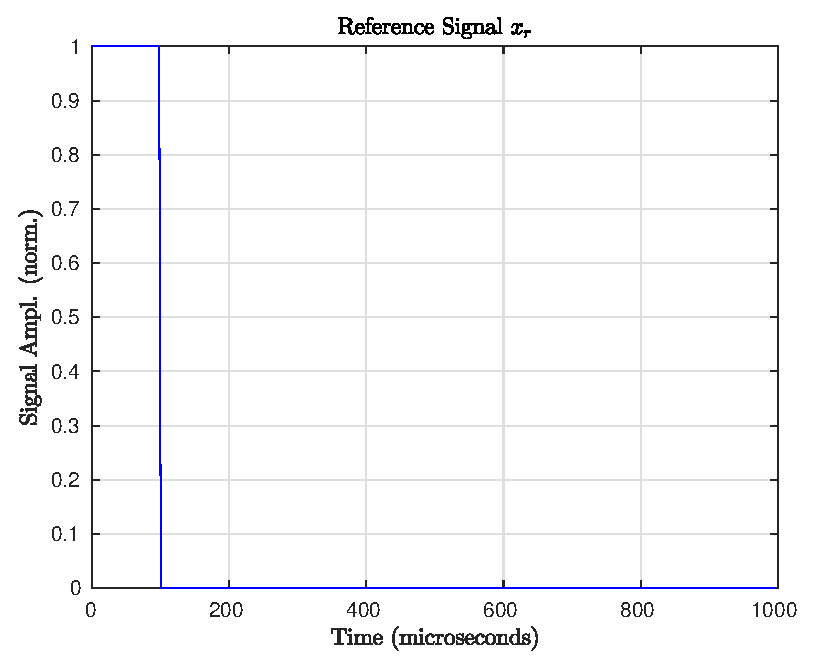
\includegraphics[width=\linewidth,height=\textheight-5\baselineskip,keepaspectratio]{reference_signal.eps}
            \end{figure}
        \end{column}
        \begin{column}{0.5\textwidth}
            \begin{figure}
                \centering
                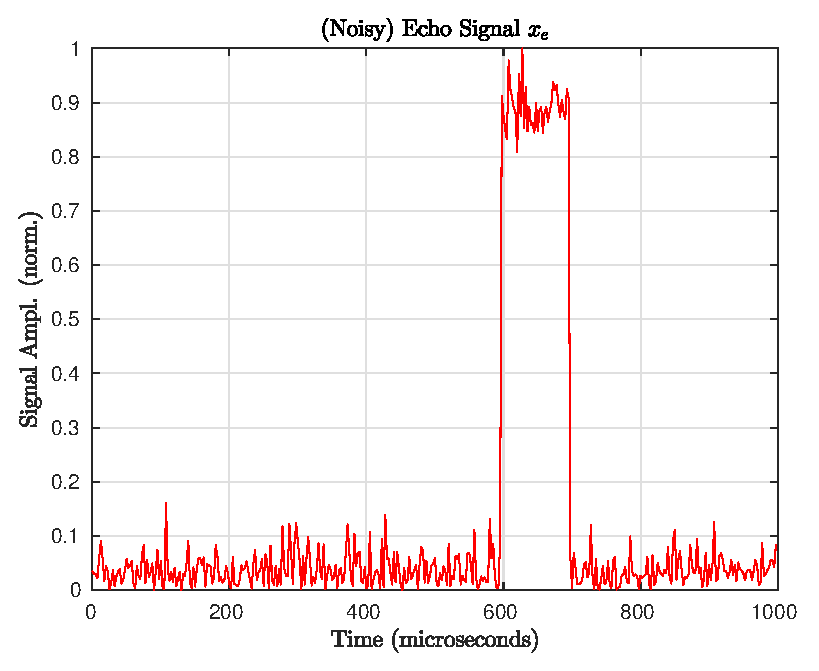
\includegraphics[width=\linewidth,height=\textheight-5\baselineskip,keepaspectratio]{echo_signal.eps}
            \end{figure}
        \end{column}
    \end{columns}
\end{frame}

\begin{frame}
    \frametitle{Kreuzkorrelation}

    \begin{figure}
        \centering
        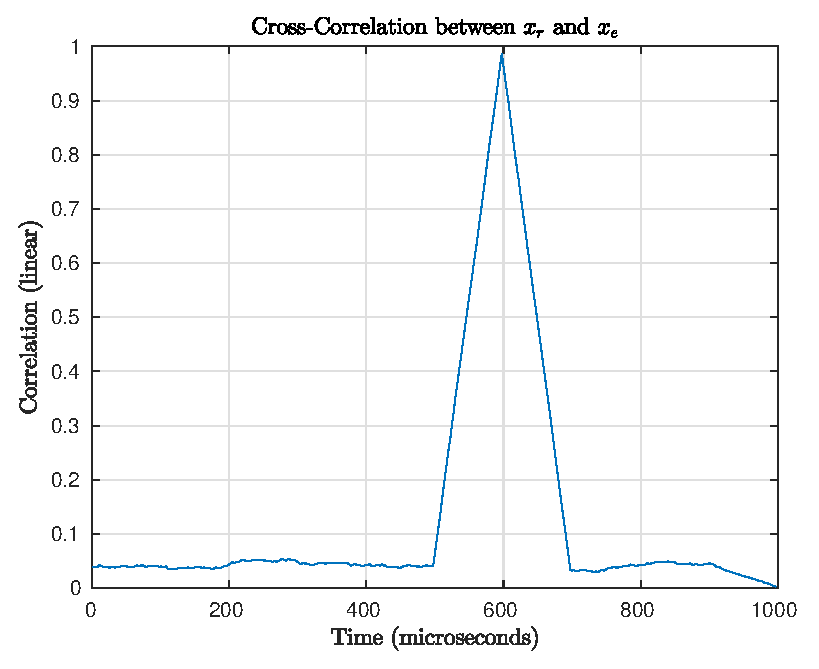
\includegraphics[width=\linewidth,height=\textheight-3\baselineskip,keepaspectratio]{correlation_linear.eps}
    \end{figure}
\end{frame}

\begin{frame}
    \frametitle{Range-Doppler Map}

    \begin{figure}
        \centering
        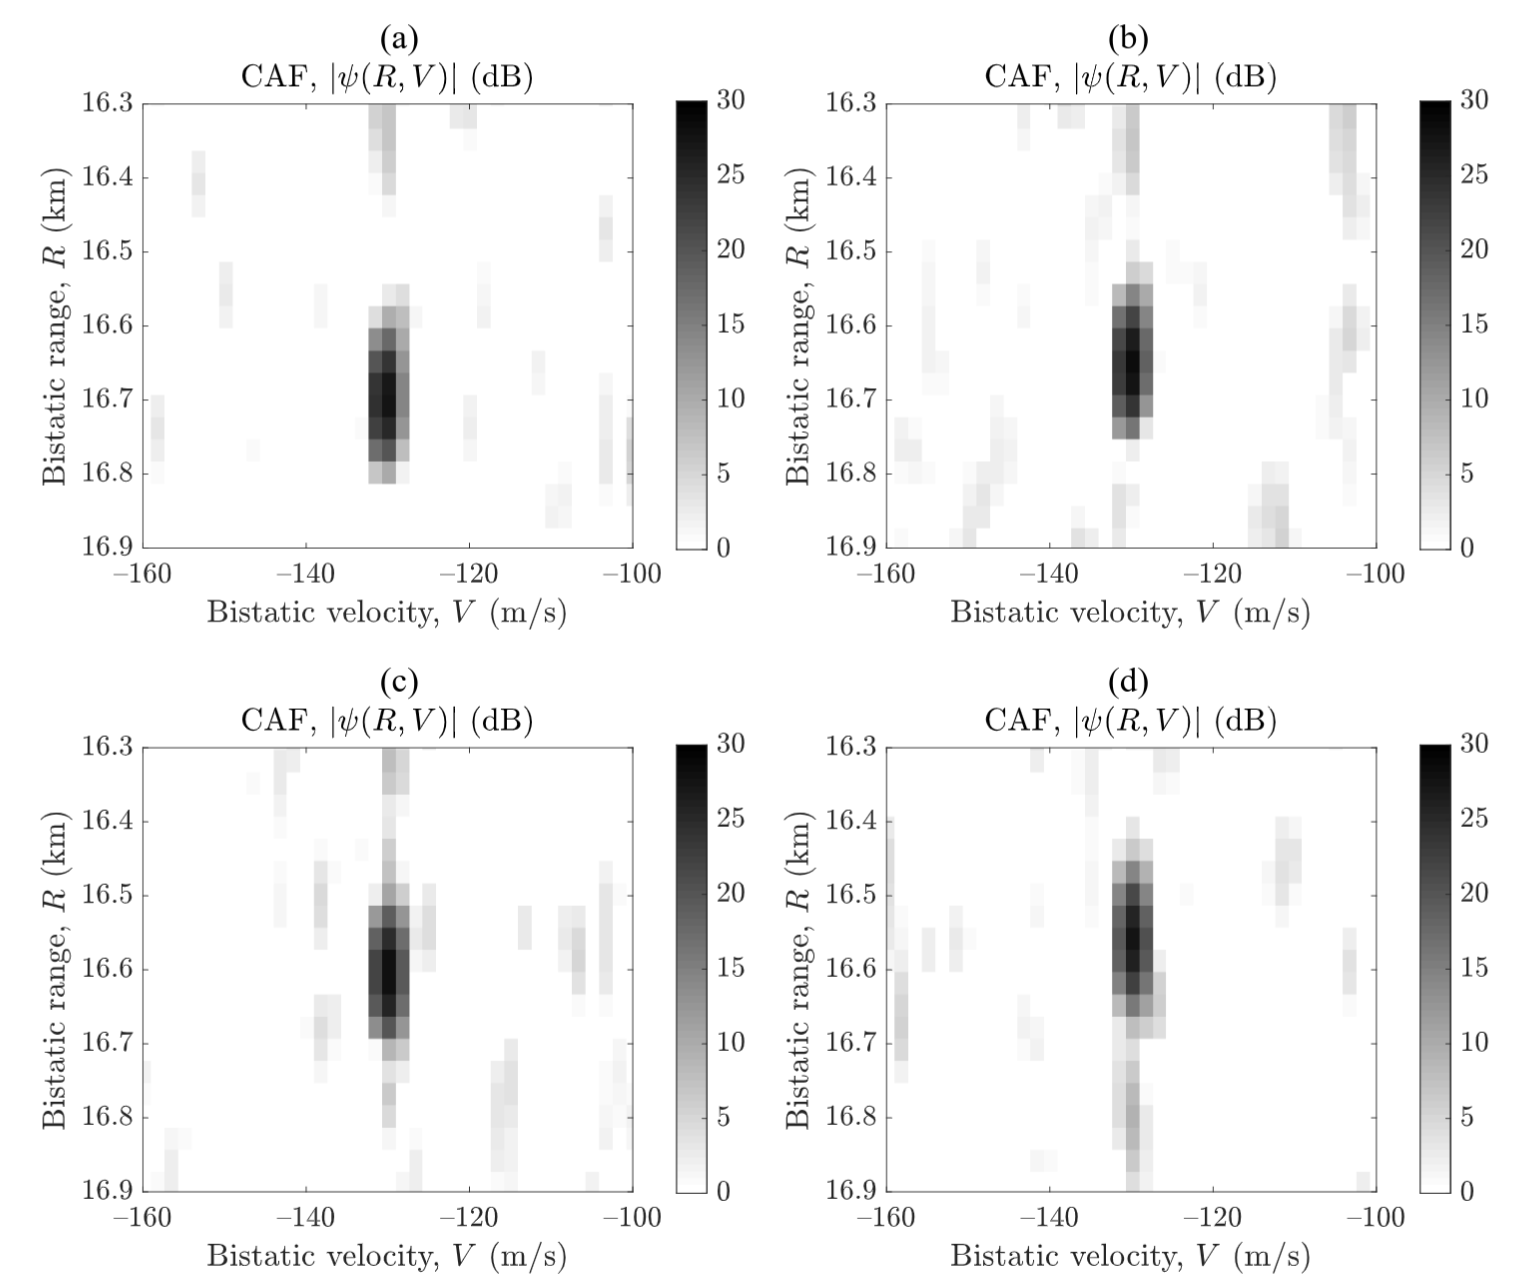
\includegraphics[width=\linewidth,height=\textheight-5\baselineskip,keepaspectratio]{range_doppler.png}
        \caption{Ausschnitt aus Kreuzambiguitätsfunktion für bewegtes Ziel~\cite[p.~161]{Malanowski2019}.}
    \end{figure}
\end{frame}

\begin{frame}
    \frametitle{Transformation in Kartesische Koordinaten}

    \Large Wie gelangt man von \textbf{bistatischer} zur \textbf{kartesischen Darstellung}?\normalsize

    \vspace{2\baselineskip}

    Möglichkeiten:
    \begin{enumerate}
        \item \textbf{Antennenrichtwirkung} nutzen um bistatischen Ellipsoiden \emph{abzutasten}
        \item \textbf{Ellipsoiden} verschiedener Rx-Tx Paare \textbf{übereinanderlegen}
    \end{enumerate}
\end{frame}

\begin{frame}
    \frametitle{Schnittpunkte der bistatischen Ellipse}

    \begin{figure}
        \centering
        \begin{adjustbox}{max width=\linewidth,totalheight=\textheight-5\baselineskip}
            \begin{tikzpicture}
                
\def\F{5}
\coordinate (rx1_coord) at (-\F,0);
\coordinate (tx1_coord) at (\F,0);
\coordinate (tx2_coord) at (2,2);
\coordinate (tx3_coord) at (1,-3);
\coordinate (target_coord) at (2,3.5);

\draw [visible on=<2->]
let
\p1=(tx1_coord),
\p2=($(target_coord)-(\p1)$),
\p3=($(target_coord)-(rx1_coord)$),
\p4=($(\p1)-(rx1_coord)$),
\n1={scalar((veclen(\x2,\y2) + veclen(\x3,\y3))*1pt/1cm)},
\n2={scalar(veclen(\x4,\y4)*1pt/1cm)},
\n3={sqrt(pow(\n1/2, 2))},
\n4={sqrt(pow(\n1/2, 2) - pow(\n2/2, 2))},
in
($(rx1_coord)!0.5!(\p1)$)
circle [x radius=\n3,y radius=\n4,draw=gray];

\draw [visible on=<3->]
let
\p1=(tx2_coord),
\p2=($(target_coord)-(\p1)$),
\p3=($(target_coord)-(rx1_coord)$),
\p4=($(\p1)-(rx1_coord)$),
\n1={scalar((veclen(\x2,\y2) + veclen(\x3,\y3))*1pt/1cm)},
\n2={scalar(veclen(\x4,\y4)*1pt/1cm)},
\n3={sqrt(pow(\n1/2, 2))},
\n4={sqrt(pow(\n1/2, 2) - pow(\n2/2, 2))},
in
($(rx1_coord)!0.5!(\p1)$)
circle [x radius=\n3,y radius=\n4,draw=gray,rotate=15.94];

\draw [visible on=<4->]
let
\p1=(tx3_coord),
\p2=($(target_coord)-(\p1)$),
\p3=($(target_coord)-(rx1_coord)$),
\p4=($(\p1)-(rx1_coord)$),
\n1={scalar((veclen(\x2,\y2) + veclen(\x3,\y3))*1pt/1cm)},
\n2={scalar(veclen(\x4,\y4)*1pt/1cm)},
\n3={sqrt(pow(\n1/2, 2))},
\n4={sqrt(pow(\n1/2, 2) - pow(\n2/2, 2))},
in
($(rx1_coord)!0.5!(\p1)$)
circle [x radius=\n3,y radius=\n4,draw=gray,rotate=-26.57];

\draw [dotted] (rx1_coord) node [cross out,draw,solid] {} node [below=2pt] {Rx}  -- (tx1_coord) node [cross out,draw,solid] {} node [below=2pt] {Tx1};

\draw [dotted] (rx1_coord) -- (tx2_coord) node [cross out,draw,solid] {} node [below=2pt] {Tx2};
\draw [dotted] (rx1_coord) -- (tx3_coord) node [cross out,draw,solid] {} node [below=2pt] {Tx3};

\node at (target_coord) [visible on=<1>] {\faPlane};
\node at (target_coord) [visible on=<4>] {\faPlane};

            \end{tikzpicture}
        \end{adjustbox}
        \caption{Schnittpunktmethode}
    \end{figure}
\end{frame}

  % !TeX root = ../beamer.tex
\section{Zusammenfassung}

\begin{frame}
    \frametitle{Zusammenfassung}

    \begin{columns}
        \begin{column}{0.4\textwidth}
            \begin{itemize}
                \item Begriffsdefinition Passivradar
                \item Monostatische und bistatische Geometrie
                \item Bistatische Entfernung und Geschwindigkeit
                \item Methode zur Bestimmung der bistatischen Entf.\ und Geschw.
            \end{itemize}
        \end{column}
        \begin{column}{0.6\textwidth}
            \centering
            \begin{adjustbox}{max width=\linewidth,max height=0.3\textheight}
                \begin{tikzpicture}
                    \newcommand\drawTopology[4]{
    \coordinate (rx1_coord) at (-2,0);
    \coordinate (tx1_coord) at (2,0);
    \coordinate (target_coord) at (1.25,3);

    \node at (tx1_coord) [text width=0.5cm,text height=1cm] (tx) {};
    \node at (tx1_coord) [antenna,scale=0.5,below=-0.5cm] {};
    \path let \p1=(tx.north west), \p2=(tx.south east), \p3=(tx) in [label={below:Receiver}] ({\x3-0.4cm},\y1) rectangle ({\x3+0.4cm},\y2) node [below] at (\x3,\y2) {Illuminator};

    \node at (rx1_coord) [text width=0.5cm,text height=0.75cm] (rx) {};
    \node at (rx1_coord) [antenna,scale=0.5,below=-0.5cm] {};
    \path let \p1=(tx.north west), \p2=(tx.south east), \p3=(rx) in [label={below:Receiver}] ({\x3-0.4cm},\y1) rectangle ({\x3+0.4cm},\y2) node [below] at (\x3,\y2) {Receiver};

    \node at (target_coord) [label={above:Target}] (target) {\Huge\faPlane};

    \draw [visible on={#1},decorate,decoration={expanding waves,angle=35,segment length=4pt},blue!60] (tx) -- (target);
    \draw [visible on={#2},decorate,decoration={expanding waves,angle=25,segment length=4pt},red!60] (target) -- node [#4] {\small\contourlength{2pt}\contour{#3}{Echo}} (rx);
    \draw [visible on={#1},decorate,decoration={expanding waves,angle=15,segment length=4pt},blue!60] (tx) -- node [#4] {\small\contourlength{2pt}\contour{#3}{Reference}} (rx);
}

                    \drawTopology{<1->}{<1->}{bg}{fg}
                \end{tikzpicture}
            \end{adjustbox}
            \begin{adjustbox}{max width=\linewidth,max height=0.3\textheight}
                \begin{tikzpicture}
                    % !TeX root = ../main.tex
\coordinate (rx1_coord) at (-2,0);
\coordinate (tx1_coord) at (2,0);
\coordinate (target_coord) at (1,1.25);

\node at (tx1_coord) [draw,fill=white] (tx1) {Tx};

\node at (rx1_coord) [draw,fill=white] (rx) {Rx};

\begin{scope}
    \clip
    let
    \p1=(target_coord),
    in
    (\x1 - 0.75cm,\y1 + 0.75cm) rectangle +(1.5,-1.5);
    \draw [color=gray]
    (2.42539052968,0) arc [start angle=0,end angle=360,x radius=2.42539052968,y radius=1.37204927807];
\end{scope}

\node at (target_coord) [label={[fill=white]above:Target}] (target) {\faPlane};

\draw [->,color=red] (tx1) -- node [black,midway,right,align=center] {$R_1$} (target);
\draw [->,color=red] (target) -- node [black,midway,left=4pt,align=center] {$R_2$} (rx);
\draw [->,color=blue] (tx1) -- node [black,midway,below,align=center] {$R_{\text{b}}$} (rx);

\pic [draw,angle radius=1cm,"$\beta$"] {angle=rx1_coord--target_coord--tx1_coord};

                    \drawBistaticGeometry{bg}
                \end{tikzpicture}
            \end{adjustbox}
            \begin{adjustbox}{max width=\linewidth,max height=0.25\textheight}
                \begin{tikzpicture}
                    
\def\F{5}
\coordinate (l_foci_coord) at (-\F,0);
\coordinate (r_foci_coord) at (\F,0);
\coordinate (point_on_ellipse_coord) at (6,0);

\draw (0,0)
let
\p1=($(point_on_ellipse_coord)-(r_foci_coord)$),
\p2=($(point_on_ellipse_coord)-(l_foci_coord)$),
\n1={scalar((veclen(\x1,\y1) + veclen(\x2,\y2))*1pt/1cm)},
\n2={\n1/2},
\n3={sqrt(pow(\n1/2, 2) - pow(\F, 2))}
in
circle [x radius=\n2,y radius=\n3,draw=gray];

\draw [dotted] (l_foci_coord) node [cross out,draw,solid] {} -- (0,0) node {\contour{bg}{$R_{\text{b}}$}} -- (r_foci_coord) node [cross out,draw,solid] {};

\foreach \u in {-5.5,-5,...,5.5} {
        \draw [->,blue] let
        \p1=($(point_on_ellipse_coord)-(r_foci_coord)$),
        \p2=($(point_on_ellipse_coord)-(l_foci_coord)$),
        \n1={scalar((veclen(\x1,\y1) + veclen(\x2,\y2))*1pt/1cm)},
        \p3=(\u,{sqrt( (pow(2 * \F / \n1, 2) - 1) * pow(\u, 2) + pow(\n1 / 2, 2) - pow(\F, 2) )}),
        \p4=($(\p3)!1cm!(l_foci_coord)$),
        \p5=($(\p3)!1cm!(r_foci_coord)$),
        \p6=($(\p4) + (\p5) - (\p3)$),
        in
        (\p3) -- ($(\p6)!1.5!(\p3)$);
    }

\foreach \u in {-6,6} {
        \draw [->,blue] let
        \p1=(\u,0),
        \p2=($(\p1)!1cm!(l_foci_coord)$),
        \p3=($(\p1)!1cm!(r_foci_coord)$),
        \p4=($(\p2) + (\p3) - (\p1)$),
        in
        (\p1) -- ($(\p4)!1.5!(\p1)$);
    }

\foreach \u in {-5.5,-5,...,5.5} {
        \draw [->,blue] let
        \p1=($(point_on_ellipse_coord)-(r_foci_coord)$),
        \p2=($(point_on_ellipse_coord)-(l_foci_coord)$),
        \n1={scalar((veclen(\x1,\y1) + veclen(\x2,\y2))*1pt/1cm)},
        \p3=(\u,{-sqrt( (pow(2 * \F / \n1, 2) - 1) * pow(\u, 2) + pow(\n1 / 2, 2) - pow(\F, 2) )}),
        \p4=($(\p3)!1cm!(l_foci_coord)$),
        \p5=($(\p3)!1cm!(r_foci_coord)$),
        \p6=($(\p4) + (\p5) - (\p3)$),
        in
        (\p3) -- ($(\p6)!1.5!(\p3)$);
    }

                \end{tikzpicture}
            \end{adjustbox}
            \tiny\begin{equation}
                \psi(R, V) = \int_{-T/2}^{T/2} {x_{e}(s) \cdot x_{r}^{*}} \left( s - \frac{R}{c} \right)\mathrm{e}^{- \mathrm{j} \frac{2 \pi}{\lambda} V s} \, d s
            \end{equation}\normalsize
        \end{column}
    \end{columns}

    \vspace{\baselineskip}

    \centering
    \huge Danke für Ihre Aufmerksamkeit! \normalsize
\end{frame}


  \begin{frame}[allowframebreaks]
    \frametitle{Quellen}
    \printbibliography
  \end{frame}

  %\appendix
  %\section{BACKUP}
  %% !TeX root = ../beamer.tex
\section{Kreuzkorrelation in Formeln}

\begin{frame}
    \frametitle{Kreuzkorrelation}

    \begin{itemize}
        \item Gibt Aussage über \textbf{Zeitversatz} zweier Signale
        \item Definition für Referenzsignal \(x_{r}\) und Echosignal \(x_{e}\):
              \begin{equation}
                  \psi(t) = \int_{-T/2}^{T/2}{ x_{e}(s) x_{r}^{*}(s - t) \, d s}
              \end{equation}
        \item<2-> Ausgedrückt als bistatische Entfernung (\(R = c t\)):
              \begin{equation}
                  \psi(R) = \int_{-T/2}^{T/2}{ x_{e}(s) x_{r}^{*} \left( s - \frac{R}{c} \right) \, d s}
              \end{equation}
        \item<3-> Wird über \textbf{Bereich von \(R\)} ausgewertet
    \end{itemize}
\end{frame}

\begin{frame}
    \frametitle{Nächster Schritt: Kreuzambiguitätsfunktion}

    \begin{itemize}
        \item Definition:
              \begin{equation}
                  \psi(R, V) = \int_{-T/2}^{T/2} {x_{e}(s) \cdot x_{r}^{*}} \left( s - \frac{R}{c} \right)\mathrm{e}^{- \mathrm{j} \frac{2 \pi}{\lambda} V s} \, d s
              \end{equation}
        \item Berücksichtigt auch \textbf{Dopplershift} und damit bistatische Geschw.
        \item Wird über \textbf{Bereich von \(R\) und \(V\)} ausgewertet
    \end{itemize}
\end{frame}

\section{Geschichte}

\begin{frame}
    \frametitle{Das Daventry Experiment}

    \begin{columns}
        \begin{column}{0.5\textwidth}
            \begin{itemize}
                \item \textbf{Passives} Radar
                \item BBC Sendeturm als Beleuchter
                \item Detektion von Bomber-Flugzeug
            \end{itemize}
        \end{column}
        \begin{column}{0.5\textwidth}
            \begin{figure}
                \centering
                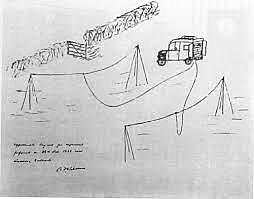
\includegraphics[width=\linewidth{},height=\textheight{}-3cm,keepaspectratio]{daventry_experiment.jpg}
                \caption{Skizze des Daventry Experiments von 1935~\cite{WattsonWatt1935}.}
            \end{figure}
        \end{column}
    \end{columns}
\end{frame}

\begin{frame}
    \frametitle{Chain Home}

    \begin{columns}
        \begin{column}{0.5\textwidth}
            \begin{itemize}
                \item Aktives Radar
                \item Nutzung während des 2. Weltkriegs
                \item Frühwarnradar gegen deutsche Luftangriffe
                \item Erste Inbetriebnahme 1937
            \end{itemize}
        \end{column}
        \begin{column}{0.5\textwidth}
            \begin{figure}
                \centering
                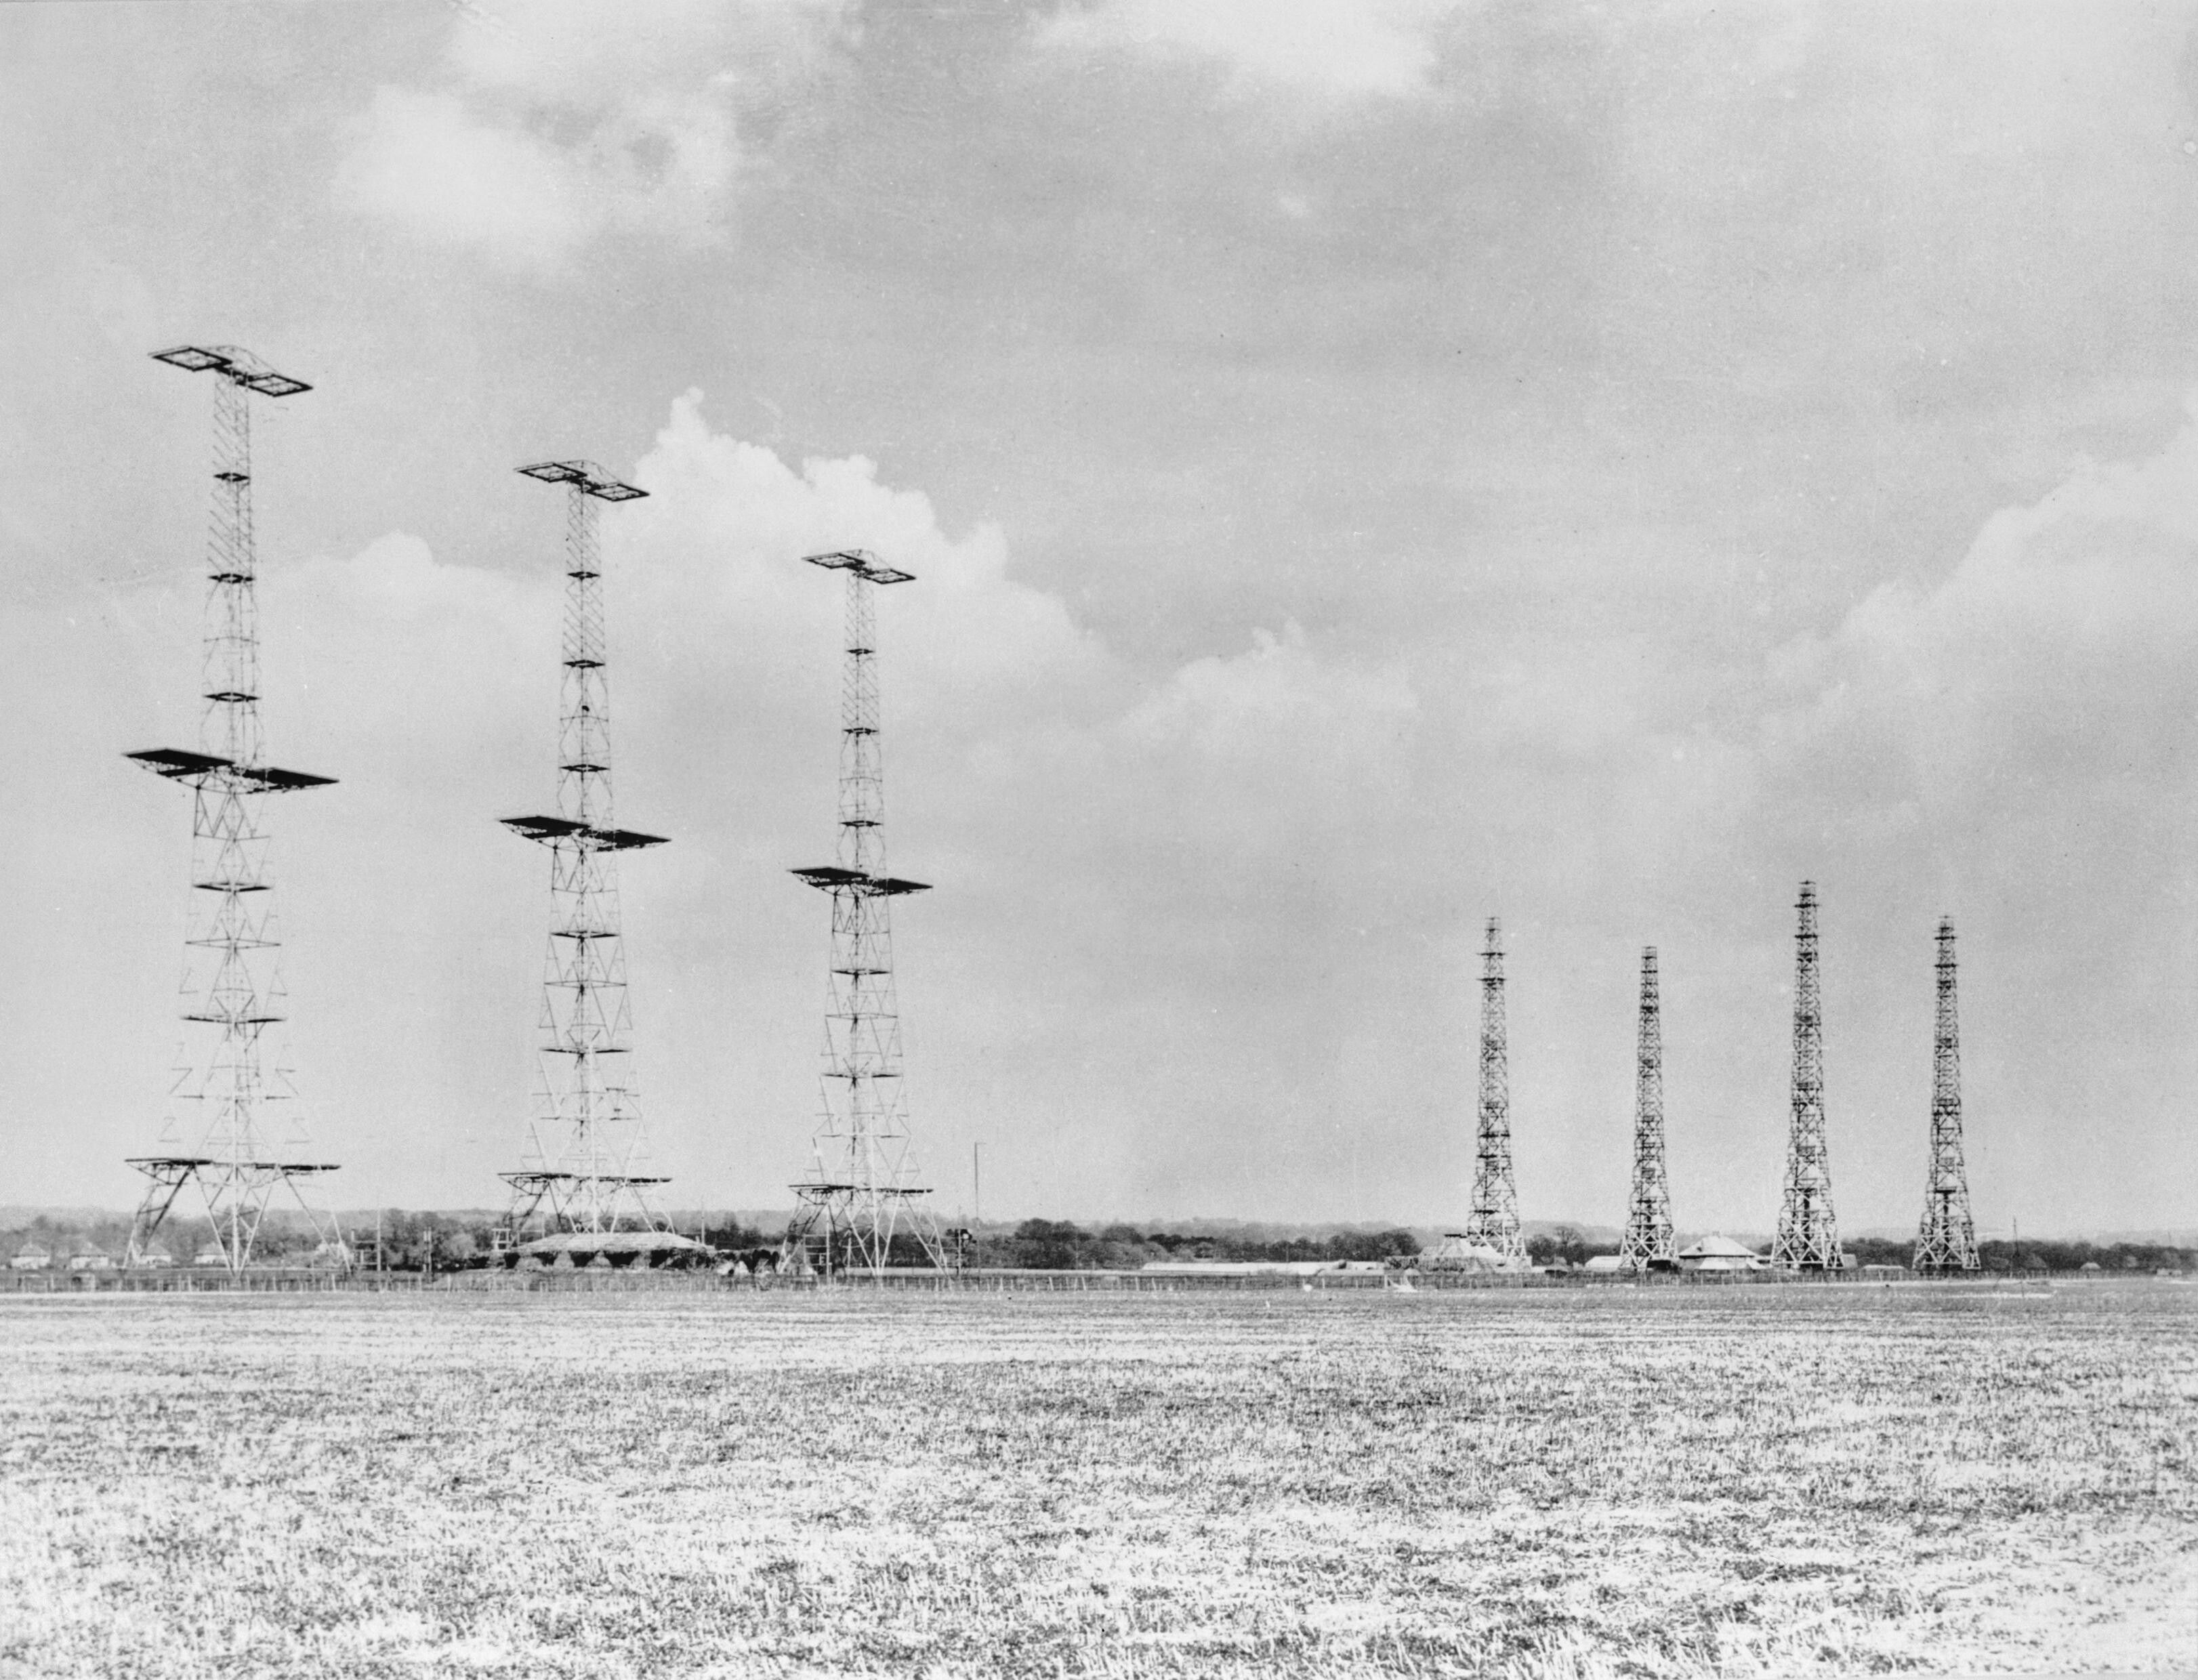
\includegraphics[width=\linewidth{},height=\textheight{}-3cm,keepaspectratio]{chain_home.jpg}
                \caption{Chain Home Antennen der Royal Airforce. Foto 1945~\cite{RoyalAirForce1945}.}
            \end{figure}
        \end{column}
    \end{columns}
\end{frame}

\begin{frame}
    \frametitle{Klein Heidelberg}

    \begin{columns}
        \begin{column}{0.44\textwidth}
            \begin{figure}
                \centering
                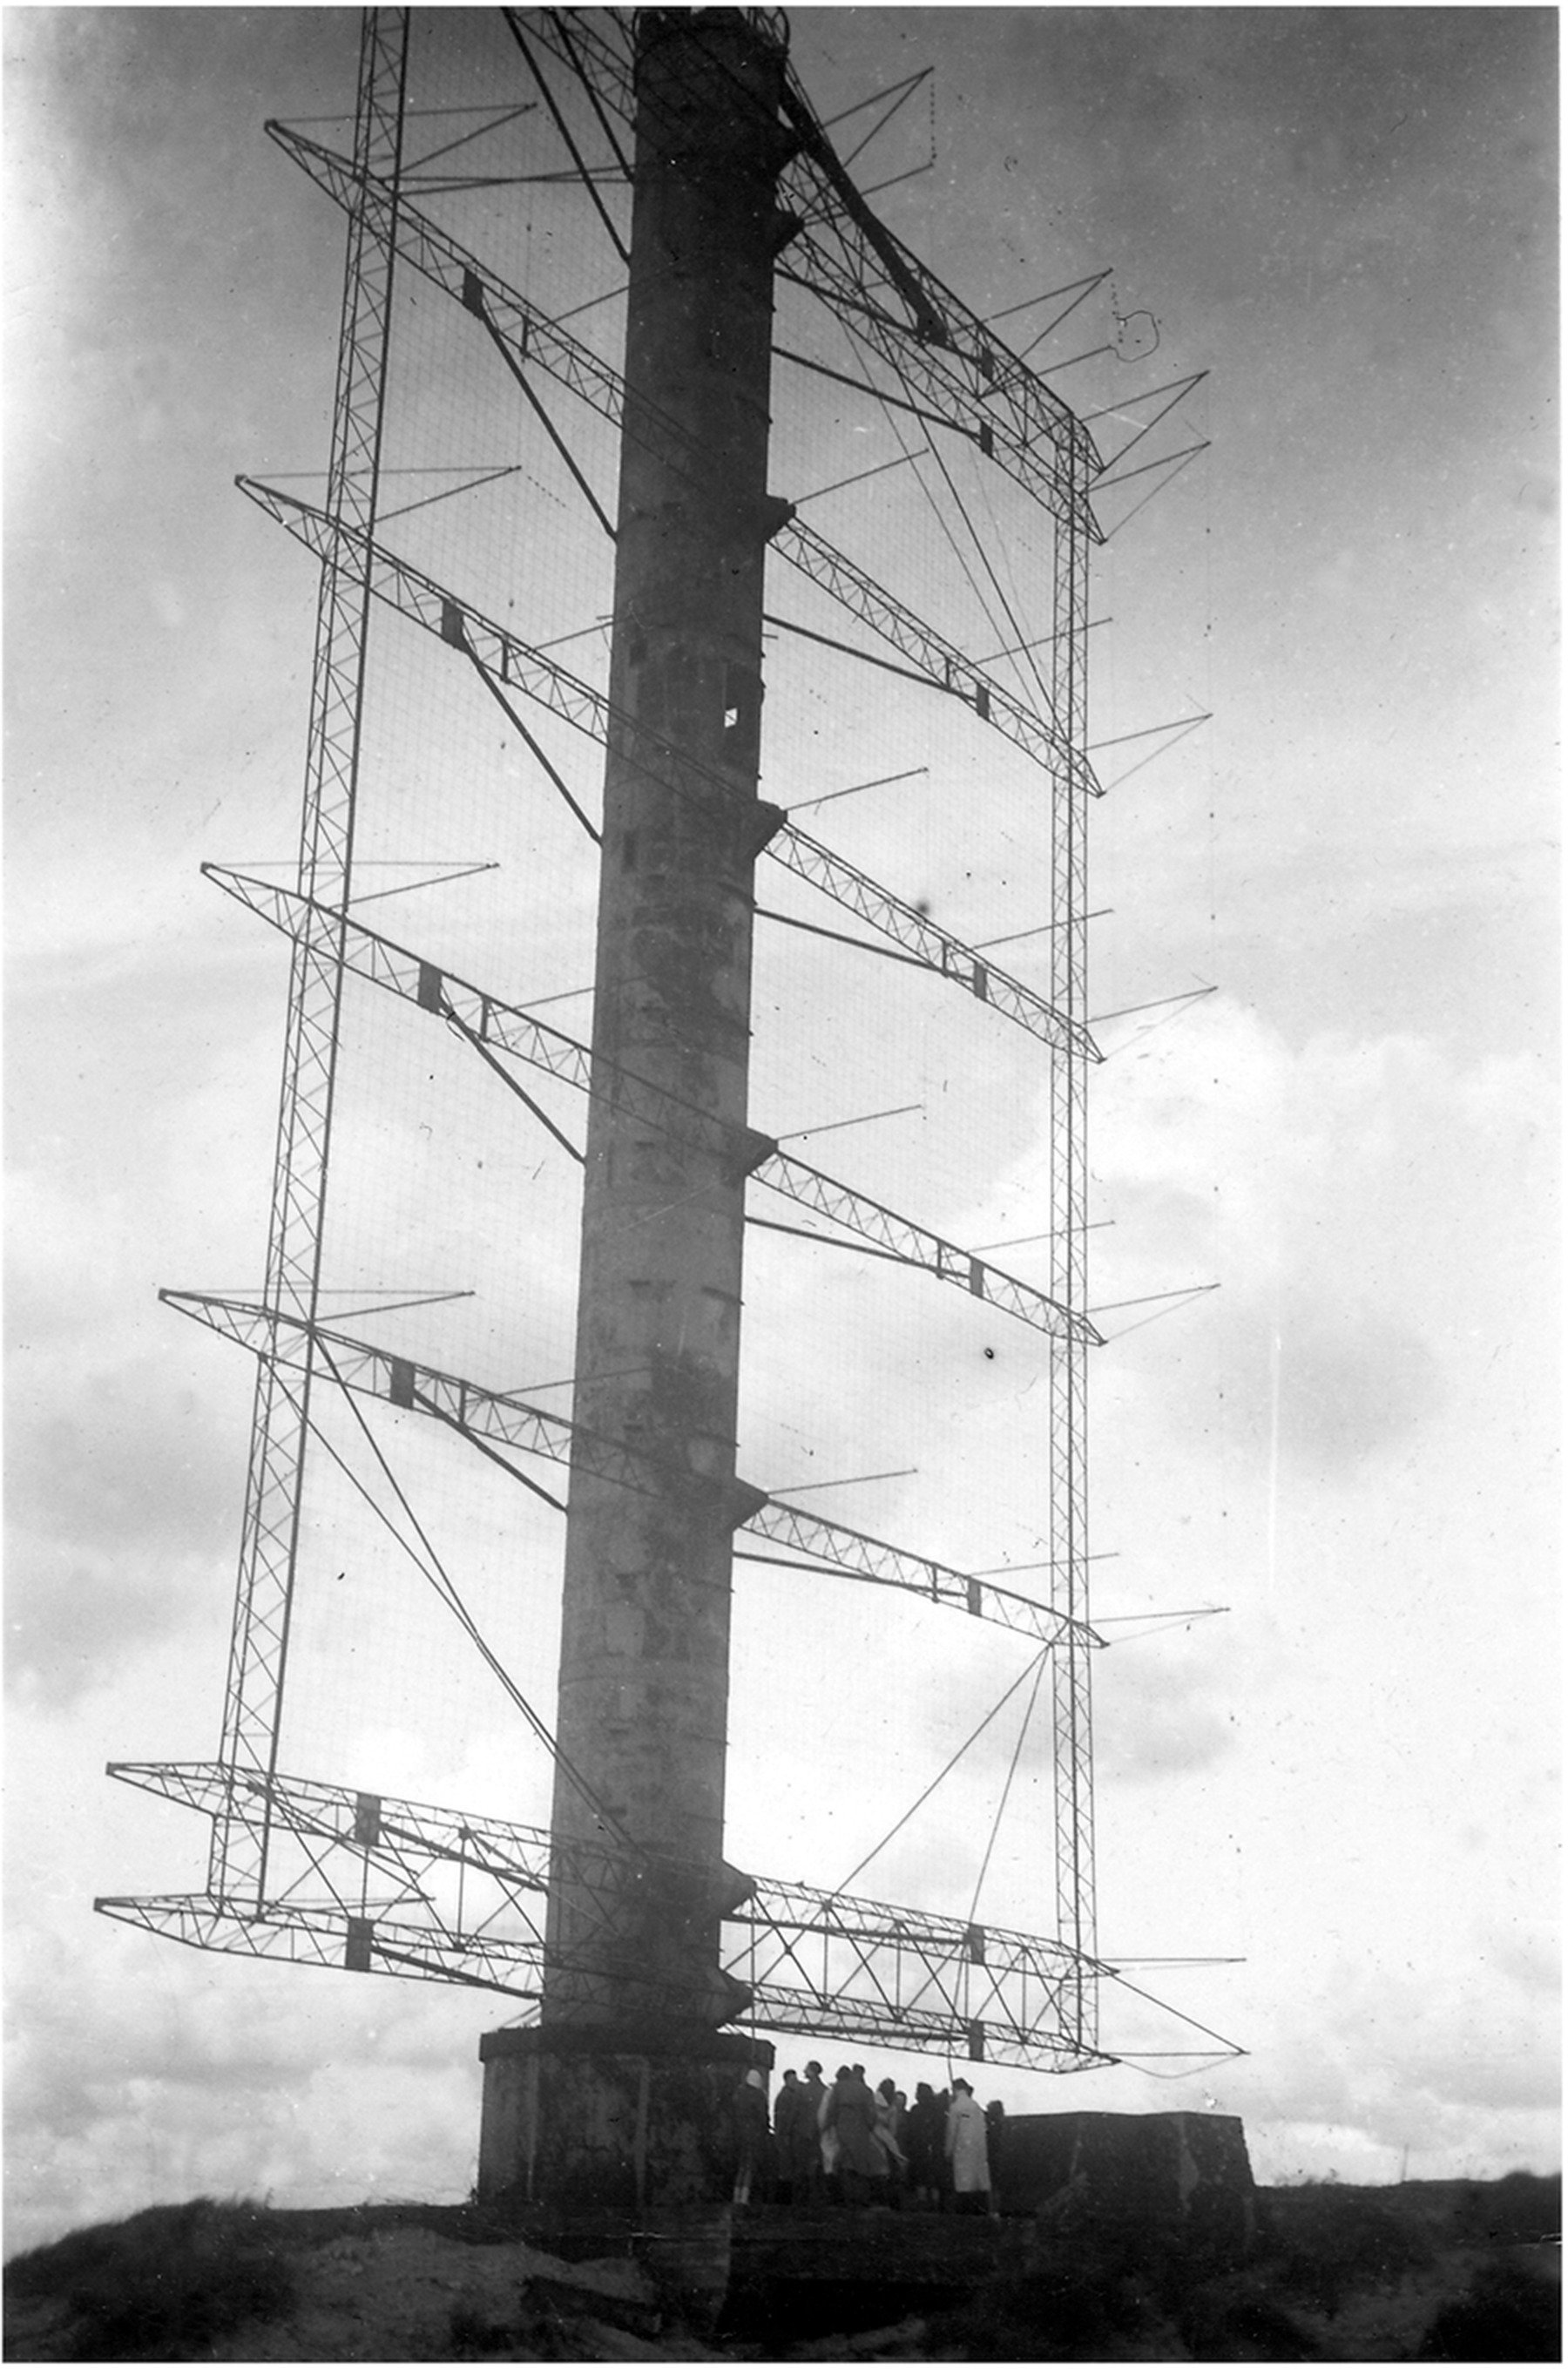
\includegraphics[width=\linewidth{},height=\textheight{}-3.5cm,keepaspectratio]{klein_heidelberg.jpg}
                \caption{Antenne des Klein Heidelberg Empfängers BIEBER (Oostvoorne, NL). Foto 1947~\cite{Rijpsma2005} as cited in~\cite{Griffiths2010}.}
            \end{figure}
        \end{column}
        \begin{column}{0.56\textwidth}
            \begin{itemize}
                \item \textbf{Passives} Radar
                \item Detektion von britischen Bombern über dem Ärmelkanal
                \item Nutzte \textbf{britisches Chain-Home} als Beleuchter
                \item Fertigstellung 1942
            \end{itemize}
        \end{column}
    \end{columns}
\end{frame}

\begin{frame}
    \frametitle{Neuzeit}

    \begin{columns}
        \begin{column}{0.55\textwidth}
            \begin{figure}
                \centering
                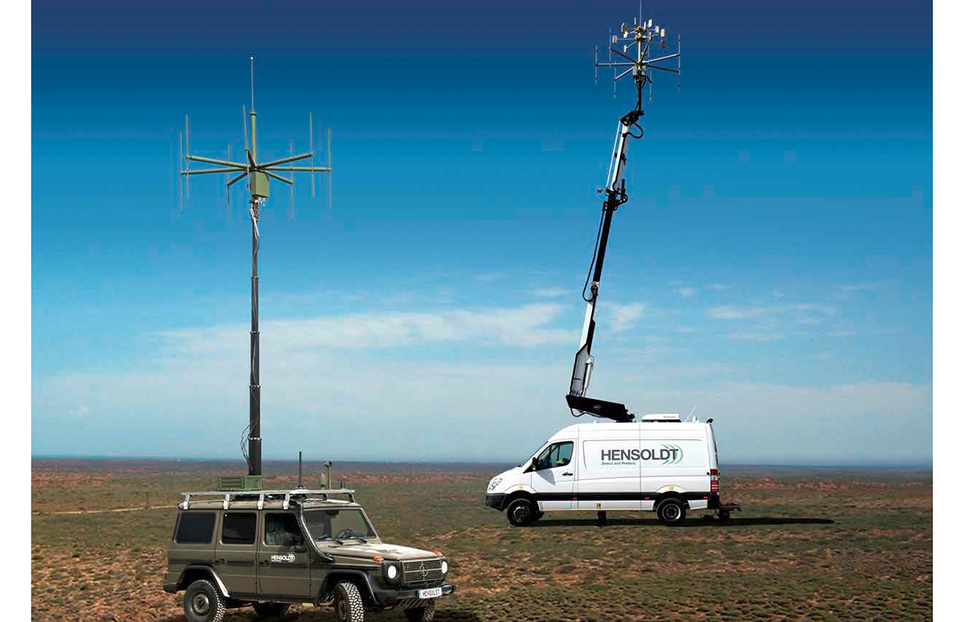
\includegraphics[width=\linewidth{},height=\textheight{}-3cm,keepaspectratio]{twinvis.png}
                \caption{TwInvis®. Modernes Passivradarsystem des Unternehmens Hensoldt~\cite{Hensoldt2019}.}
            \end{figure}
        \end{column}
        \begin{column}{0.45\textwidth}
            \begin{itemize}
                \item Zunächst basierend auf FM Beleuchtern
                \item Später DAB und DVB-T
                \item GSM, LTE
                \item \dots
            \end{itemize}
        \end{column}
    \end{columns}
\end{frame}

\section{Beleuchtungsquellen}

\begin{frame}
    \frametitle{Beleuchtungsquellen (Illuminators of Opportunity)}

    \begin{columns}
        \begin{column}{0.2\textwidth}
            \begin{figure}
                \raggedleft{}
                \begin{tikzpicture}
                    \begin{axis}[
                            ymode=log,
                            height=6cm,
                            width=2cm,
                            hide x axis,
                            axis y line=left,
                            ymin=1,
                            ymax=100,
                            ylabel={Entfernung [\si{\kilo\metre}]},
                        ]
                        \addplot [draw=none] {1};
                    \end{axis}
                \end{tikzpicture}
            \end{figure}
        \end{column}
        \begin{column}{0.8\textwidth}
            \begin{itemize}
                \item FM-Radio
                \item DVB-T (Digitales Fernsehen)
                \item DAB (Digitales Radio)
                \item LTE
                \item GSM
                \item WiFi
            \end{itemize}
        \end{column}
    \end{columns}
\end{frame}

}

\end{document}
